\documentclass{beamer}

\mode<presentation>
{\usetheme{boxes}}

\usepackage{array}
\usepackage{times}
\usepackage{graphicx}
\usepackage{hyperref}
\usepackage{listings}
\usepackage{relsize}
\usepackage{ragged2e}
\usepackage[T1]{fontenc}

\lstdefinestyle{customc}{
  belowcaptionskip=1\baselineskip,
  breaklines=true,
  frame=L,
  xleftmargin=\parindent,
  language=C,
  showstringspaces=false,
  basicstyle=\footnotesize\ttfamily,
  keywordstyle=\bfseries\color{green!40!black},
  commentstyle=\itshape\color{purple!40!black},
  identifierstyle=\color{blue},
  stringstyle=\color{red},
}
\lstdefinestyle{custombash}{
  belowcaptionskip=1\baselineskip,
  breaklines=true,
  frame=L,
  xleftmargin=\parindent,
  language=bash,
  basicstyle=\footnotesize\ttfamily,
  showstringspaces=false,
  commentstyle=\itshape\color{purple!40!black},
  keywordstyle=\itshape\color{green!40!black},
  identifierstyle=\color{blue},
  stringstyle=\color{orange},
}

\usebackgroundtemplate
{
  \hbox to \paperwidth{\hfil
\includegraphics[width=4in,
      height=\paperheight]{wildcat_transparent.jpg}\hfil}
}

\title{PHYS 105 Lecture 9: File I/O, Histograms}
\author{Tom McClintock \\
	Dept. of Physics\\
	University of Arizona
}
\date{\today}

\begin{document}

\begin{frame}
  \titlepage
\end{frame}

\begin{frame}
  \frametitle{Last time}
  \begin{itemize}
    \item Graphics
    \item Random numbers
    \item Random walk
  \end{itemize}
\end{frame}

\begin{frame}
  \frametitle{This time}
  \begin{itemize}
    \item File I/O
    \item Histograms
  \end{itemize}
\end{frame}

\begin{frame}
  \frametitle{File output}
  Oftentimes it is more useful to write the output of a program into a file
  rather than onto the terminal. Some reasons for this include:
  \begin{itemize}
    \item Too much output
    \item Output gets saved
    \item Need the output as input for another program
  \end{itemize}
  In this class we are going to create some data and save it to a file 
  that we will use later in the semester.
\end{frame}

\begin{frame}[fragile]
  \frametitle{Quick example of writing to a file}
  You start by creating a file pointer \textbf{fp} to an open file.
  Then you can write to the file using \textbf{fprintf()}:
  \begin{lstlisting}[style=customc]
    FILE* fp = fopen(``test.txt'',``w'');
    fprintf(fp, ``this text is in the file\n'');
  \end{lstlisting}
  Then, once you run your program you can see the file with \textbf{ls}:
  \begin{lstlisting}[style=custombash]
    ls
  \end{lstlisting}
  You can see what is in the file with the command \textbf{less}:
  \begin{lstlisting}[style=custombash]
    less test.txt
  \end{lstlisting}
  Quit \textbf{less} by typing 'q'.
\end{frame}

\begin{frame}
  \frametitle{fileout.c}
  Here is a quick example.
  \lstinputlisting[style=customc]{fileout.c}
  
\end{frame}

\begin{frame}[fragile]
  \frametitle{Data for analysis}
  We will use our random walk code to create data. Specifically, we want to run the program
  many, many times and keep track of how far the walker gets from the starting position.\\
  Later in the semester we will analyse this output and visualize it in a variety of ways.\\
  Let's copy our random walk code into a new file:
  \begin{lstlisting}[style=custombash]
    cp randomwalk.c manywalks.c
    ls
\end{lstlisting}
\end{frame}

\begin{frame}[fragile,allowframebreaks]
  \frametitle{manywalks.c}
  NOTE: the graphical portion of the random walk was removed.
  \lstinputlisting[style=customc]{manywalks.c}
\end{frame}

\begin{frame}[fragile]
  \frametitle{Inspecting the output file}
  Let's take a look at the file we create with this.
  \begin{lstlisting}[style=custombash]
    ls
    less outfile.txt
  \end{lstlisting}
  Quit \textbf{less} by typing 'q'.
\end{frame}

\begin{frame}[fragile]
  \frametitle{File input}
  The compliment to file output is file input, or reading from files.\\
  Just like how output required us to use \textbf{fprintf()}, to do
  file input we use \textbf{fscanf()}.
  \begin{lstlisting}[style=customc]
    int var; //A variable used for input
    FILE* fp = fopen(``test.txt'',``r'');
    fprintf(fp, ``%i'', &var);
    ...
  \end{lstlisting}
  The above reads in a single integer into the variable \textit{var}.\\
  \vspace{12pt}
  CRITICAL NOTE: when reading in a file, you open the file pointer with ``r''.
\end{frame}

\begin{frame}[fragile]
  \frametitle{Reading in your own files}
  At the moment the only files that you have that 
  you can read from are your own files.
  Later I will provide you with real data to plot, 
  but for now you will read in the
  data from the manywalks.c program.
\end{frame}

\begin{frame}[fragile,allowframebreaks]
  \frametitle{filein.c}
  Here you will read in the file you created and print each line.
  \lstinputlisting[style=customc]{filein.c}
\end{frame}

\begin{frame}[fragile]
  \frametitle{Histograms}
  Histograms are one of the first graphs you ever learn to read.\\
  Here is some fake data describing student's grades on an assignment
  graded from 1 to 5. The elements of the \textit{Hist} array contain
  how many students got that grade.
  \begin{lstlisting}[style=customc]
    int Hist[] = {1,5,9,6,3};
  \end{lstlisting}
  \centering
  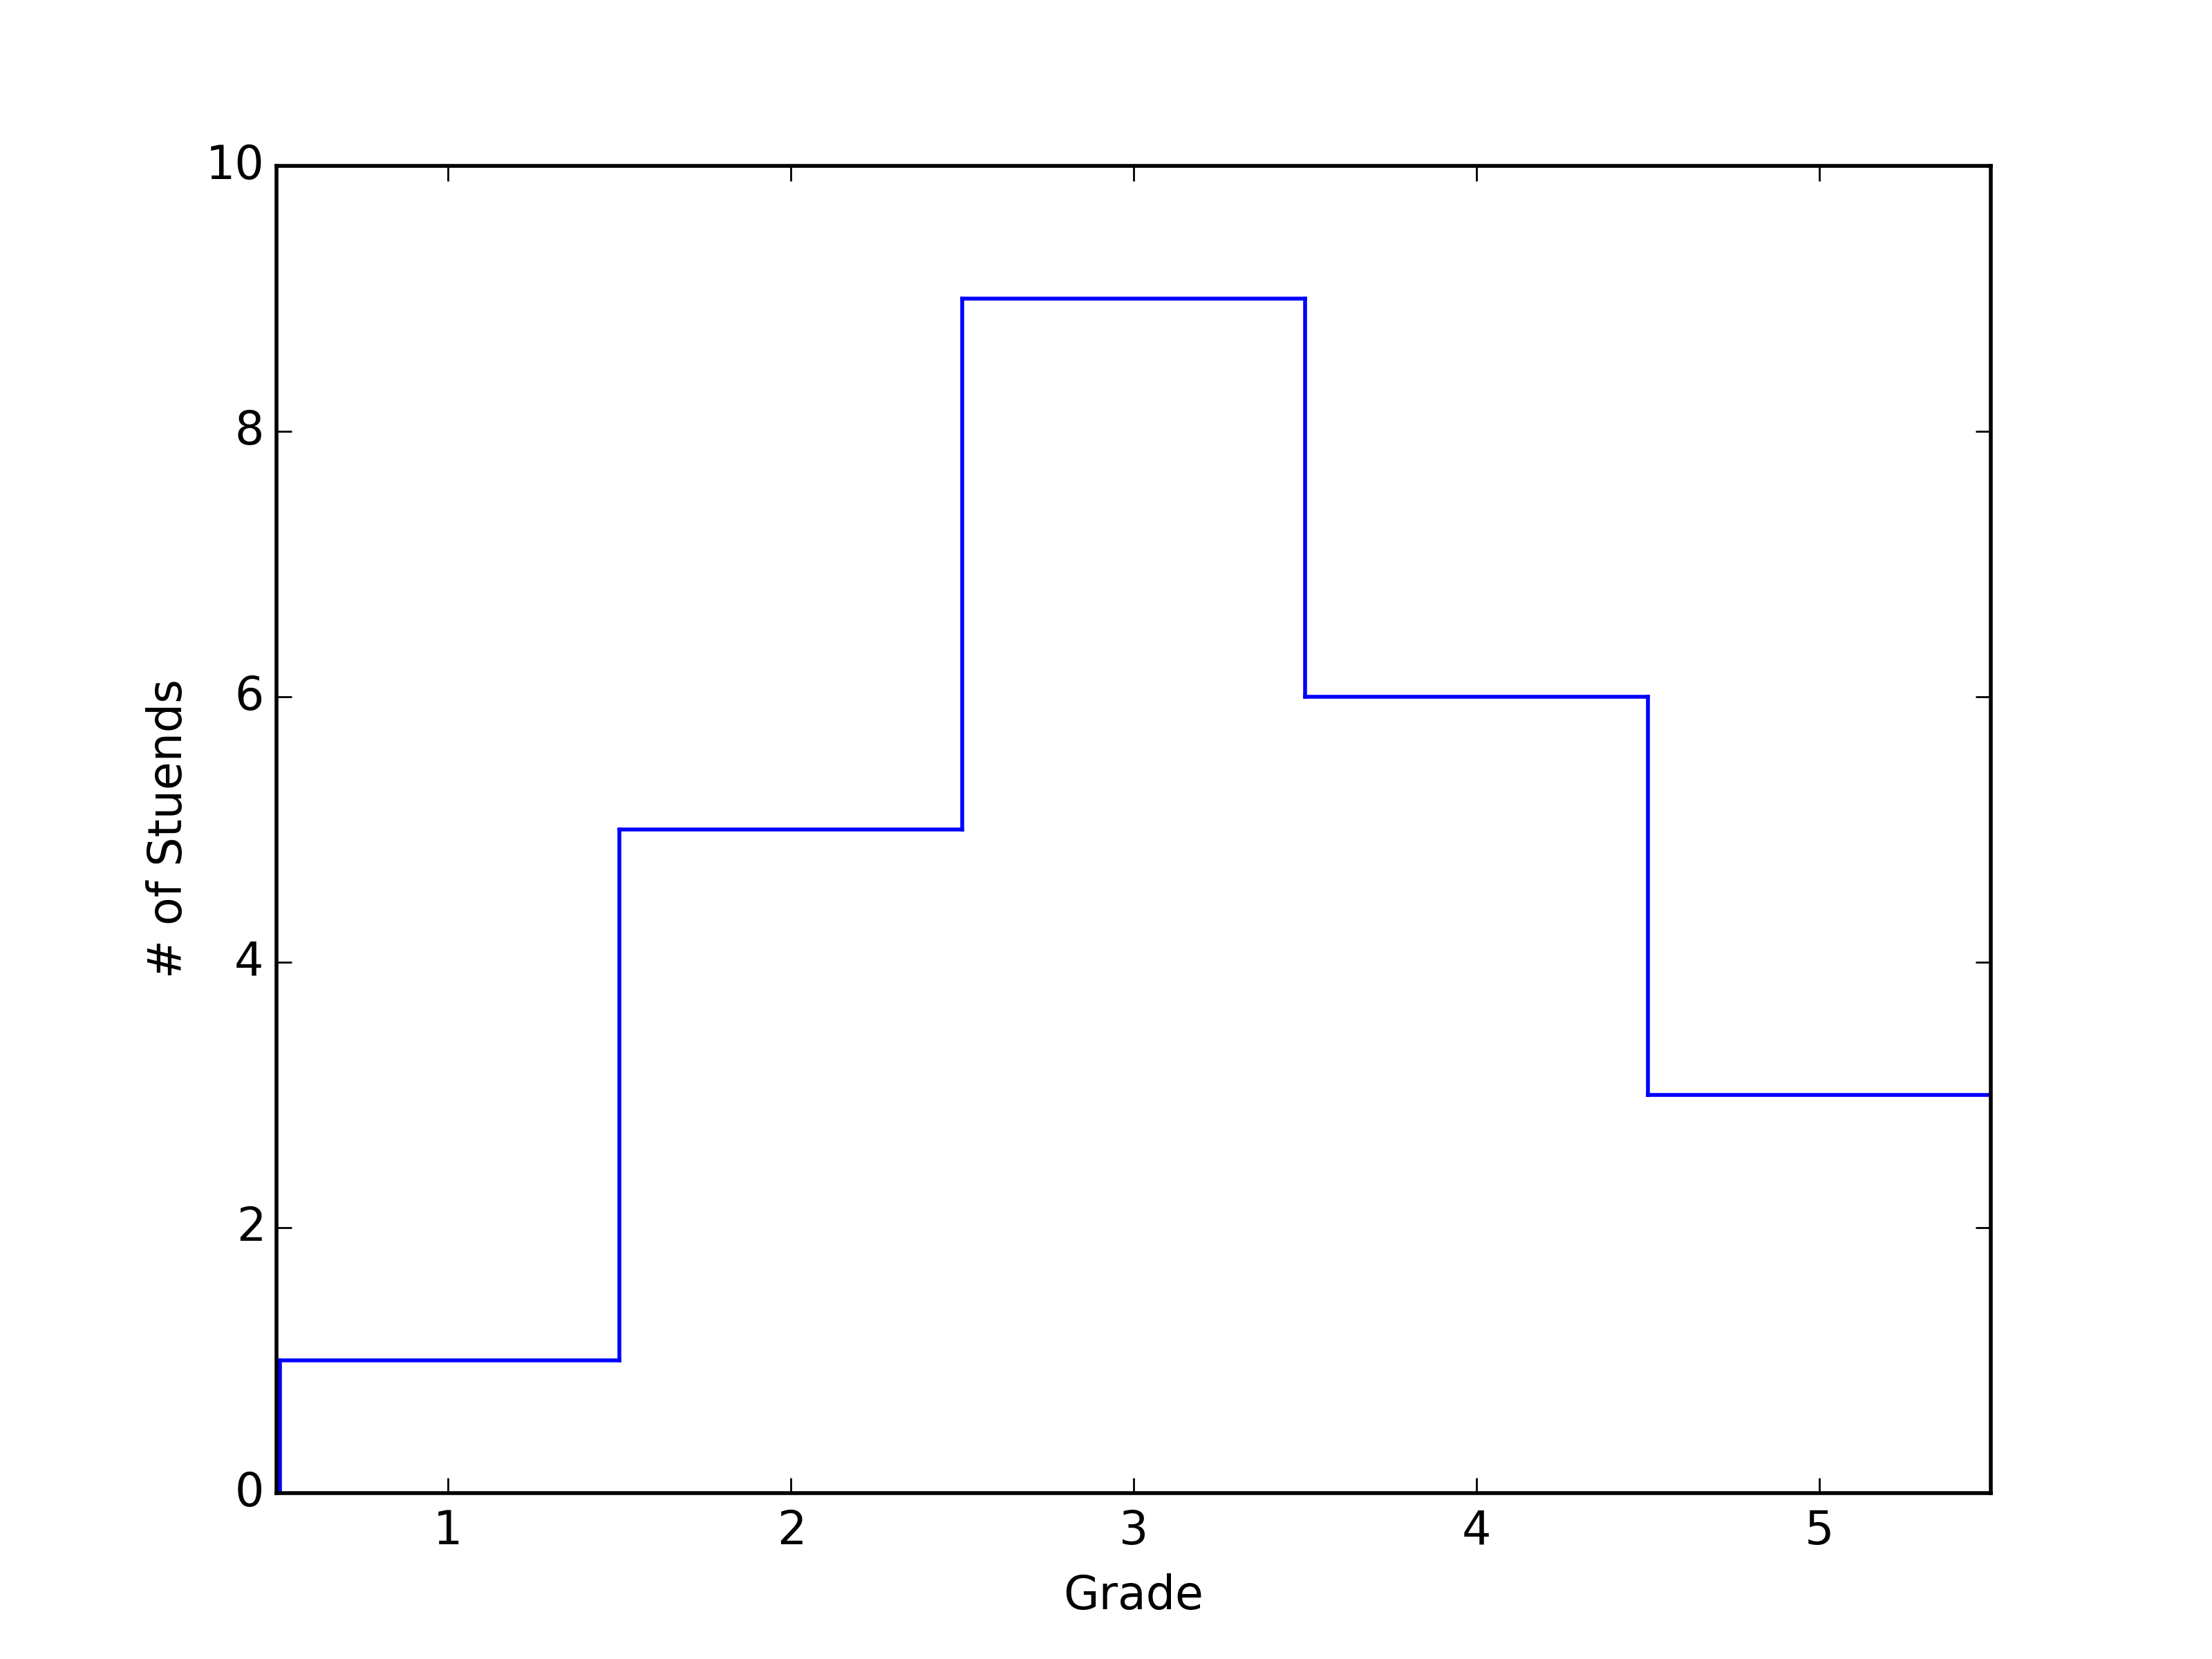
\includegraphics[width=0.7\textwidth]{histogram.png}

%  Here is some example data that I have made a histogram for:\\
%  \vspace{12pt}
%  \centering
%  UA New Students 2010-2014\\
%  \vspace{12pt}
%  \begin{tabular}{c c}
%    2010 & 8900\\
%    2011 & 9143\\
%    2012 & 9365\\
%    2013 & 8865\\
%    2014 & 9793\\
%  \end{tabular}
\end{frame}

\begin{frame}
  \frametitle{Creating a histogram}
  Histograms can be created easily in philsplot.
  \begin{enumerate}
  \item Set up a plotting window in philsplot.
  \item Call locate\_plot() at the bottom left corner of the plot.
  \item Create a for loop that loops over the number of bins. In this
    for loop:\\
    \begin{enumerate}
    \item Draw a vertical line up to the height (i.e. \textit{Hist[i]}).
    \item Draw a horizontal line across to the start of the next column.
    \end{enumerate}
  \item Flush the plot to the screen.
  \item Close the plot.
  \end{enumerate}
\end{frame}

\begin{frame}
  \frametitle{In class assignment}
  Implement the algorithm from the previous slide and reproduce the
  histogram I made.
\end{frame}

\begin{frame}
  \frametitle{Next time}
  \begin{itemize}
    \item Drawing a Gaussian
    \item Dynamic displays
  \end{itemize}
\end{frame}

\begin{frame}
  \frametitle{HW 5 - Due next week}
  Take your histogram code and now plot a histogram of the data 
  that you outputted in outfile.txt. In other words, 
  make the following alterations to the histogram code:
  \begin{enumerate}
    \item Read in your data into an array.
    \item Draw a histogram of your data.
  \end{enumerate}
  The code to draw the histogram will look identical to the in class
  assignment, and the reading in of the data will look identical
  to the program we wrote in class.
\end{frame}

\end{document}